\scanpage{221}
\inserted{dénombrable (p.ex. de t.f. sur $\mathbf Q$)}
\deleted{un \uline{\unsure{suite|corps}} de \unsure{puissance}}, on voit encore que
$\xi_{\unsure{v|\nu}}^{\mathbf Z}\simeq\xi_{\unsure{w|\omega}}^{\mathbf Z}$.
En effet, $k$ est réunion filtrante d’une \uline{suite} $A_i$ de sous-$k_0$-algèbres de type fini,
on peut supposer les morphismes de transition
$\operatorname{Spec}A_j\mathbin{—}\operatorname{Spec}A_i$
lisses à fibres géom. connexes, donc idem pour $X_j\mathbin{—}X_i$,
donc aussi pour $X_{j\mathbf C}\mathbin{—}X_{i\mathbf C}$.
On a des pts $x_i,y_i$ dans $X_{i\mathbf C}$, s’envoyant les uns sur les autres par les
morphismes de transition, et grâce à la lissité et la connexité des fibres,
on voit que les morphismes de transition
$\pi^1(x_j,y_j)\mathbin{—}\pi^1(x_i,y_i)$ sont surjectifs.
Donc $\varprojlim_i\pi^1(x_i,y_i)\ne\varnothing$, on gagne.
\figure{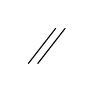
\begin{tikzpicture}\draw (0,0)--(.35,.45);\draw (.12,0)--(.47,.45);\end{tikzpicture}}
Si $k$ pas dénombrable,

2) \deleted{$E\subset k_0$ alg. fermé dans $k$.}
\inserted{$\unsure{v|\nu}$ et $\unsure{w|\omega}$ ne coïncident pas sur $E$.}
Alors je \deleted{\unsure{dis}}\inserted{pense} qu’il existe $\alpha$ tel que
\deleted{\unsure{et un motif} $M$,}
\[
 \xi_{\unsure{v|\nu}}^{\mathbf Z}|\mathcal M_\alpha(X)
 \not\simeq
 \xi_{\unsure{w|\omega}}^{\mathbf Z}|\mathcal M_\alpha(X).
\]
\margin{\deleted{$\unsure{\xi_v(M)}\ne\unsure{\xi_w(M)}$}}
On peut supposer que $X=\operatorname{Spec}\unsure{k|E}$, $k$ extension finie de $\mathbf Q$,
\deleted{\unsure{De plus}, \unsure{on peut supposer}, \unsure{pour} \illegible{4},
\unsure{que} $k$ \unsure{est} \illegible{1} \unsure{sur} $\mathbf Q$,}
\margin{220}
